\chapter{CPTAC Glioblastoma Discovery Study}
\label{chap:cptac-gbm-discov}

% This chapter describes work published at https://doi.org/10.1016/j.ccell.2021.01.006
% i need fig1, fig2a/b, fig 4 a/d-f, fig 5a, fig 7a/c.

\begin{figure}[tbp]
    \centering
    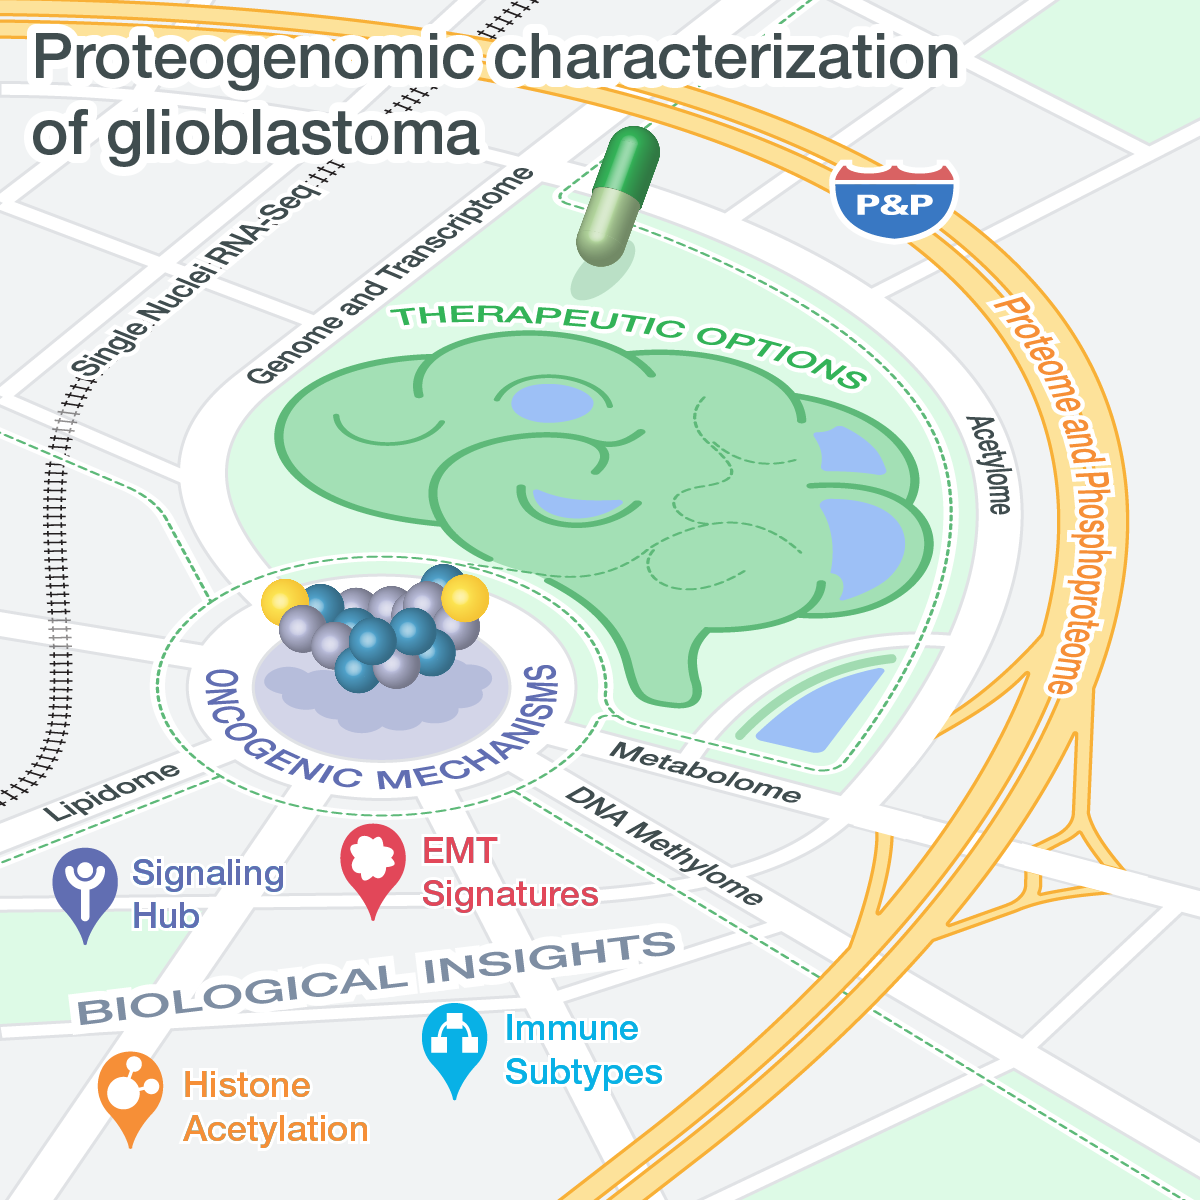
\includegraphics[width=0.5\linewidth]{figures/chap04_cptac_gbm_discov/graphical_abstract.png}
    \caption{Graphical abstract of the CPTAC GBM discovery study.}
    \label{fig:gbm-graphical-abstract}
\end{figure}

\section{Summary}
Glioblastoma (GBM) is the most aggressive nervous system cancer. Understanding its molecular pathogenesis is crucial to improving diagnosis and treatment. Integrated analysis of genomic, proteomic, post-translational modification and metabolomic data on 99 treatment-naive GBMs provides insights to GBM biology. We identify key phosphorylation events (e.g., phosphorylated PTPN11 and PLCG1) as potential switches mediating oncogenic pathway activation, as well as potential targets for \gene{EGFR}-, \gene{TP53}-, and RB1-altered tumors. Immune subtypes with distinct immune cell types are discovered using bulk omics methodologies, validated by snRNA-seq, and correlated with specific expression and histone acetylation patterns. Histone H2B acetylation in classical-like and immune-low GBM is driven largely by BRDs, CREBBP, and EP300. Integrated metabolomic and proteomic data identify specific lipid distributions across subtypes and distinct global metabolic changes in \gene{IDH}-mutated tumors. This work highlights biological relationships that could contribute to stratification of GBM patients for more effective treatment.

\section{Introduction}
Glioblastoma (GBM) is the most common primary malignant brain tumor, with roughly 12,000 new cases annually in the United States and median survival under 2 years \cite{delgado-lopezpd_corrales-garciaem:SurvivalGlioblastoma2016,ostromqt_barnholtz-sloanjs:CBTRUSStatistical2019}. The Cancer Genome Atlas (TCGA) \cite{brennancw_chinl:GBM2013,tcga_network:GBM2008} and other studies \cite{yanh_bignerdd:IDH1IDH22009} have reshaped the World Health Organization classification of nervous system tumors \cite{louisdn_ellisondw:2016World2016} to include molecular features \cite{bratdj_wellerm:CIMPACTNOWUpdate2018, louisdn_vondeimlinga:AnnouncingCIMPACTNOW2017}.
GBM is categorized as either \gene{IDH}-wild type (\gene{IDH}-WT; \textasciitilde90\%) or \gene{IDH}-mutant (\textasciitilde10\%). \gene{IDH}-WT GBMs fall into three distinct subclasses (proneural, classical, and mesenchymal) based on genomic alterations and gene expression signatures \cite{verhaakrgw_hayesdn:IntegratedGenomic2010,wangq_verhaakrgw:TumorEvolution2017}. Methylome-based classification is being used to differentially diagnose brain tumors \cite{karimis_zadehg:CentralNervous2019,nassirif_aldapekd:DNAMethylation2019} and may become clinically useful for GBM.
Surgical resection, chemotherapy, and radiotherapy remain the standard of care \cite{stuppr_mirimanoffro:RadiotherapyConcomitant2005,perryjr_trialinvestigators:ShortCourseRadiation2017}, with the recent addition of tumor treating fields \cite{stuppr_ramz:EffectTumorTreating2017}.
Promising immunotherapies have been proposed, including immune checkpoint inhibitors, vaccines, chimeric antigen receptor T cell (CAR-T) therapy, and viral therapy, though none have cleared Phase III trials \cite{limm_wellerm:CurrentState2018,mcgranahant_nagpals:CurrentState2019}.
Despite different subtypes, no specific treatment works more effectively in a pre-specified subset of patients based on transcriptomics, though those with MGMT promoter methylation respond better to temozolomide \cite{stuppr_mirimanoffro:RadiotherapyConcomitant2005}.

Here, we integrated proteogenomic and metabolomic data from 10 platforms including whole genome sequencing (WGS), whole exome sequencing (WES), RNA sequencing (RNA-seq), microRNA-seq (miRNA-seq), single nuclei RNA-seq (snRNA-seq), DNA methylation arrays, proteome, phosphoproteome, acetylome, lipidome, and metabolome to investigate 99 treatment-naive GBMs prospectively collected by the Clinical Proteomic Tumor Analysis Consortium (CPTAC). We report new immune-based subtypes, activation of DNA repair pathways via upregulated phosphosite levels of DNA repair genes in \gene{TP53}-mutated tumors, an apparent phospho-signaling bottleneck in receptor tyrosine kinase (RTK)-altered tumors, and enrichment of histone H2B acetylation and low macrophage content in classical-like GBM tumors. We used single-cell data to investigate contributions of various cell types to bulk tumor signatures and analyzed the mesenchymal subtype to discern epithelial-mesenchymal transition (EMT) signatures in tumor and infiltrating immune cells. The data presented here furnish a resource for future GBM studies.


\section{Results}

\subsection{Proteogenomic and metabolomic features delineate molecular subtypes of glioblastoma}
We characterized the proteogenomic landscape of 99 GBMs and 10 unmatched GTEx normal brain samples. This cohort has diverse origins and clinical characteristics typical of adult GBM. Six cases harbored \gene{IDH1} R132H mutations and had earlier disease onset than those with \gene{IDH1}-WT (median 47 vs. 59 years, t test p = 0.055). We detected one additional non-hotspot \gene{IDH1} mutation (R222C).

\begin{figure}[p]
    \centering
    \phantomlabel{fig:gbm-overview-data-avail}
    \phantomlabel{fig:gbm-overview-mut-landscape}
    \phantomlabel{fig:gbm-overview-multi-omics}
    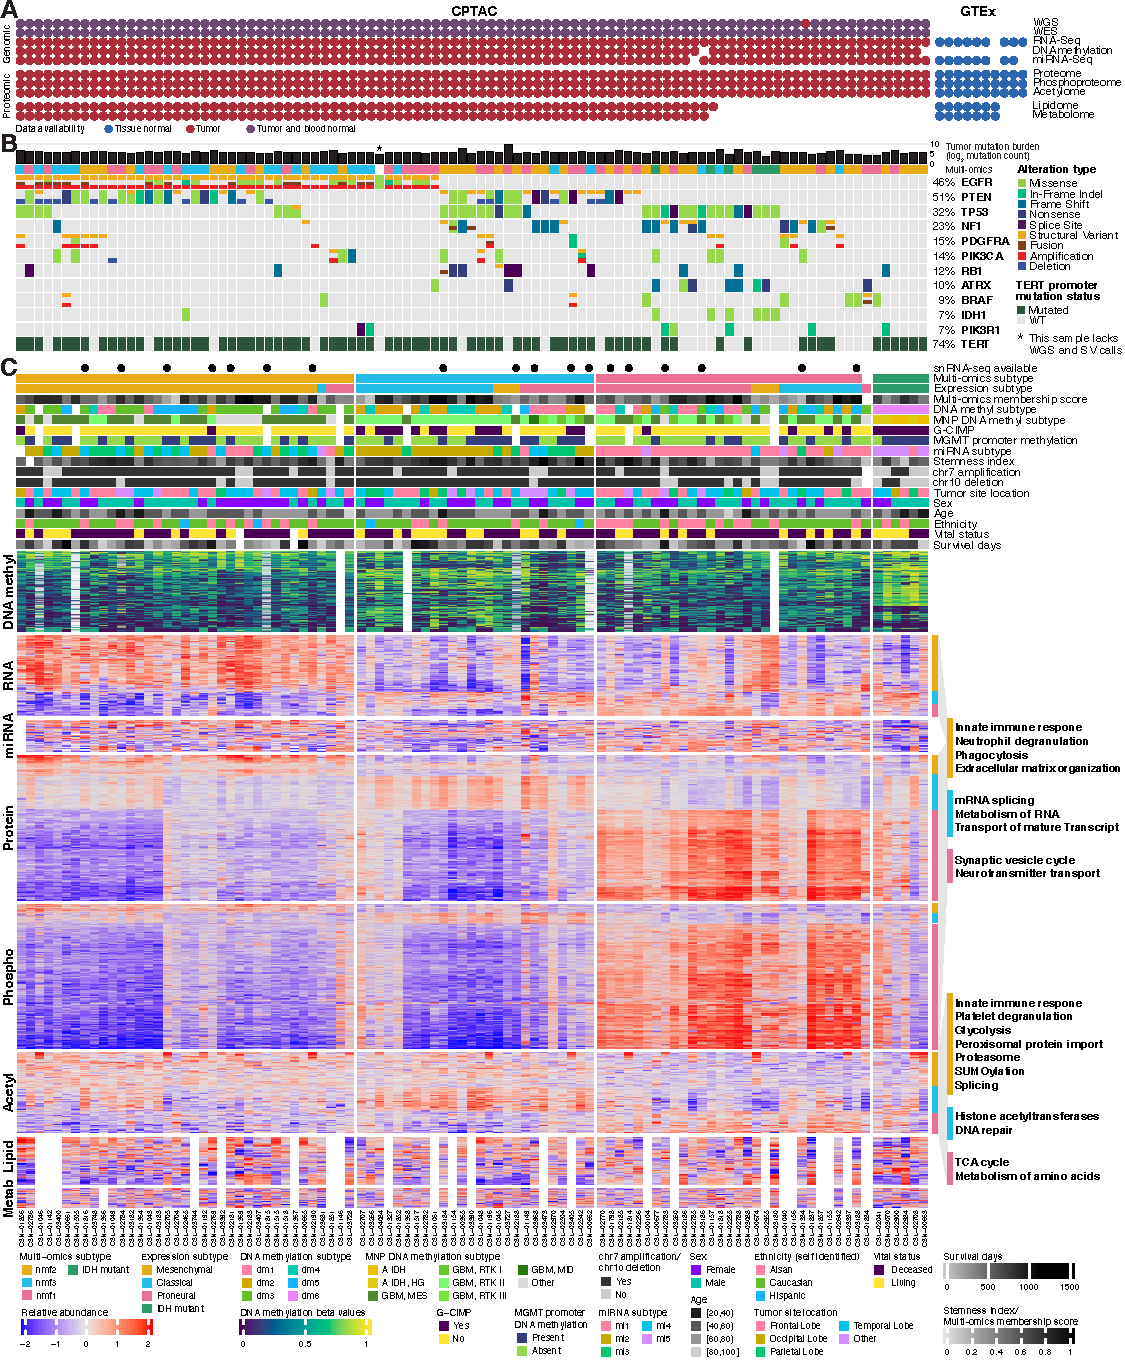
\includegraphics[width=\linewidth]{figures/chap04_cptac_gbm_discov/figure1_overview.pdf}
    \caption[Proteogenomic summary of the cohort.]{%
        Proteogenomic summary of the cohort.
        \legendcontdnote
    }
    \label{fig:gbm-overview}
\end{figure}
\begin{figure}[t]
    \centering
    \legend{%
    \legendcontdref{fig:gbm-overview}
    \subref{fig:gbm-overview-data-avail}
    Summary of 10 data types generated in this study.
    \subref{fig:gbm-overview-mut-landscape}
    Overview of significantly altered genes found in at least 5\% of samples, showing tumor mutation burden ($\log_2$ WES mutation count) and structural variants, fusions, and CNVs. Subtypes are based on results in panel \subref{fig:gbm-overview-multi-omics}.
    \subref{fig:gbm-overview-multi-omics}
    Multi-omics clustering of tumor samples by NMF using CNV, expression, and protein and phosphoprotein abundances. Heatmaps show differential expression between subtypes, including DNA methylation, acetylome, metabolome, and lipidome, and characteristic features for each subtype. Pathway enrichment analysis highlights differences between subtypes. Neuron activity related pathways, immune response pathways, and cell cycle pathways were respectively enriched in the nmf1 (proneural-like), nmf2 (mesenchymal-like), and nmf3 (classical-like) subtypes.
    }
\end{figure}

All samples were homogenized and aliquoted for each of the ten different omics assays (\fref{fig:gbm-overview-data-avail}, \ref{fig:gbm-proteomic-qc-exp-design}--\subcaptionref{fig:gbm-proteomic-qc-corr}). Mass spectrometry (MS) quantified protein, phosphorylation and acetylation, as previously described \cite{douy_zhaog:CPTACUCEC2020,mertinsp_ncicptac:CPTACBreastCancer2016} (\fref{fig:gbm-proteomic-qc-exp-design}--\subcaptionref{fig:gbm-proteomic-qc-corr}). Metabolome and lipidome levels were respectively measured by label-free gas and liquid chromatography coupled to MS. Genomic properties of our cohort were comparable to those of TCGA GBM cohort \cite{brennancw_chinl:GBM2013} (\fref{fig:gbm-overview-mut-landscape}). We identified many structural variants (SV) in oncogenes, including \gene{EGFR} and \gene{PDGFRA}, and tumor suppressors \gene{PTEN} and \gene{NF1}. \gene{EGFR} mutations often co-occurred with \gene{EGFR} SV and amplification events (p < 0.01). WES and WGS identified \gene{TERT} promoter (\gene{TERT}p) mutations with variant allele frequency (VAF) >5\% (\fref{fig:gbm-overview-mut-landscape}). Copy number analysis identified common focal and arm-level copy number variations (CNVs) (\fref{fig:gbm-subtype-gistic}).

\begin{figure}[p]
    \centering
    \phantomlabel{fig:gbm-proteomic-qc-exp-design}
    \phantomlabel{fig:gbm-proteomic-qc-prot-id}
    \phantomlabel{fig:gbm-proteomic-qc-corr}
    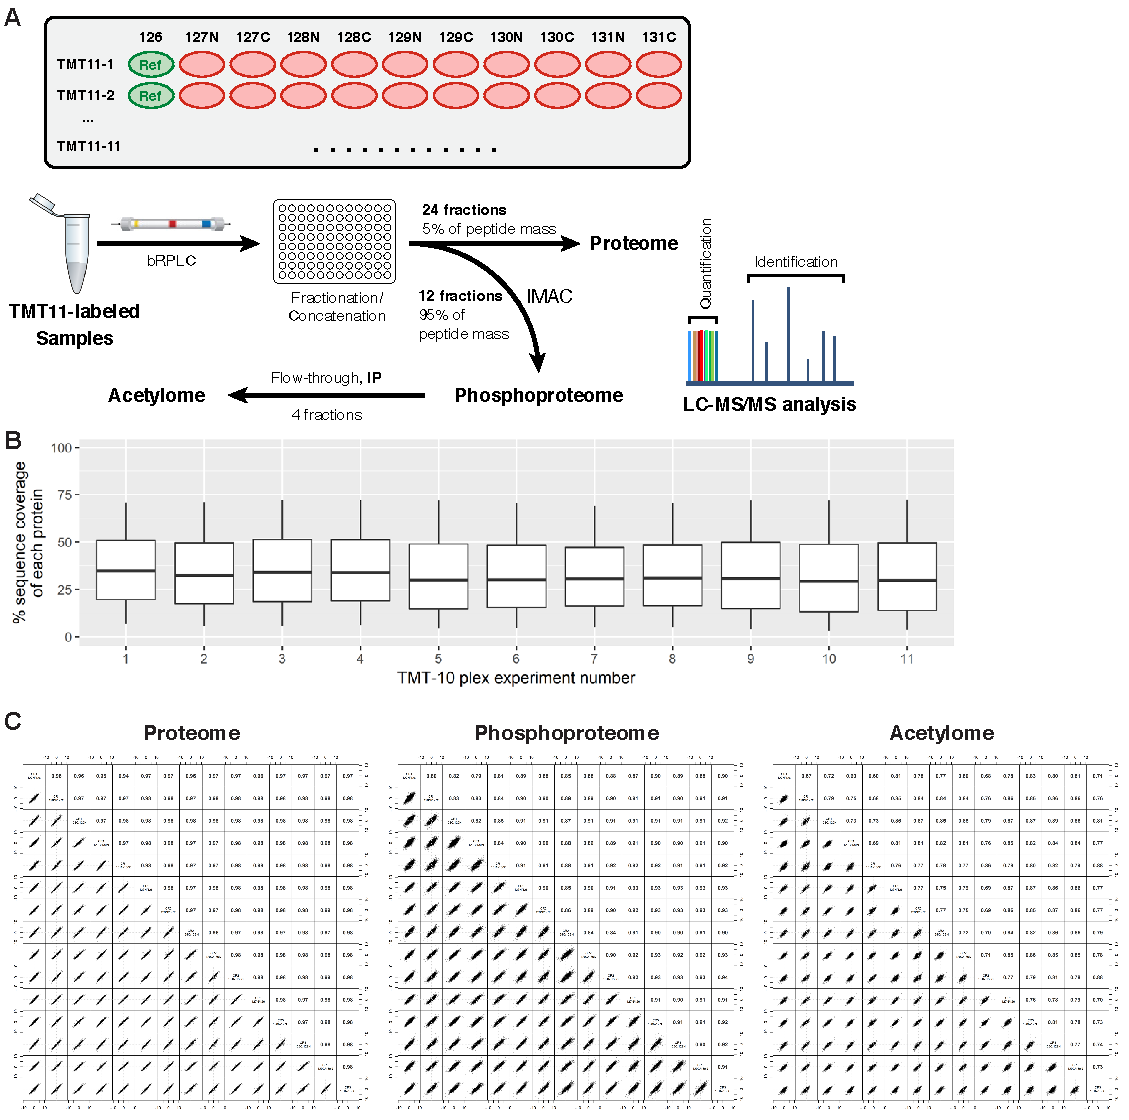
\includegraphics[width=0.9\linewidth]{figures/chap04_cptac_gbm_discov/figures1_proteome_qc.pdf}
    \caption[Integrated Proteomic Workflow and Quality Control.]{%
        Integrated Proteomic Workflow and Quality Control.
        \subref{fig:gbm-proteomic-qc-exp-design}
        TMT-11 based global proteome, phosphoproteome, and acetylome analysis workflow. The GBM tumors and GTEx normal tissues were analyzed in 11 TMT 11-plex experiments, each with 10 study samples and a common internal reference sample created by pooling all study samples (equal contribution). The TMT11-labeled samples were then fractionated, split (with 5\% peptide mass analyzed directly for global proteome), and subjected to tandem enrichment of phosphopeptides and acetylated peptides. Peptides were detected and quantified using information from the TMT-11 MS/MS spectra.
        \subref{fig:gbm-proteomic-qc-prot-id}
        Distribution of sequence coverage of the identified proteins with tryptic peptides detected by MS/MS in each TMT-11 plex; whiskers show the 5--95 percentiles. The total numbers of identified proteins in each TMT plex range from 9,992 to 10,572.
        \legendcontdnote
    }
    \label{fig:gbm-proteomic-qc}
\end{figure}
\begin{figure}[t]
    \centering
    \legend{%
        \legendcontdref{fig:gbm-proteomic-qc}
        \subref{fig:gbm-proteomic-qc-corr}
        Robust and precise proteomics platforms. Longitudinal performance was tested by repeated proteome, phosphoproteome and acetylome analysis of aliquots of the same patient-derived xenograft QC samples in standalone TMT-11 plexes, along with the GBM study samples; scatter plots and Pearson correlations comparing individual replicate measurements are shown.
    }
\end{figure}

We added protein and phosphosite abundance to prior clustering studies of gene expression (\fref{fig:gbm-overview-multi-omics}, \ref{fig:gbm-subtype}). While our results are concordant with TCGA expression-based classification \cite{wangq_verhaakrgw:TumorEvolution2017}, 27 tumors (29\%) were classified as a different subtype (\fref{fig:gbm-overview-multi-omics}, \ref{fig:gbm-subtype-nmf}).
Based on similarities with gene expression subtypes, we designated the three clusters observed in IDH-WT tumors as nmf1 (proneural-like; n = 29), nmf2 (mesenchymal-like; n = 37), and nmf3 (classical-like; n = 26).
Pathway enrichment analysis of RNA, protein, and phosphosite abundances indicated that nmf1 was enriched for synaptic vesicle cycle and neurotransmission transport; nmf2 was enriched for innate immune response, including neutrophil degranulation, phagocytosis, and extracellular matrix organization; and nmf3 was enriched for mRNA splicing and RNA metabolism.
Based on the known functional effects of protein acetylation \cite{naritat_choudharyc:FunctionsMechanisms2019}, nmf1/proneural-like cluster had a higher abundance of acetylated proteins involved in the TCA cycle and metabolism of amino acids, whereas the nmf2/mesenchymal-like cluster was enriched for innate immune system activation, peroxisomal protein import and glycolysis. The nmf3/classical-like subtype was enriched for acetylation of chromatin modifiers and DNA repair proteins.

\begin{figure}[p]
    \centering
    \phantomlabel{fig:gbm-subtype-gistic}
    \phantomlabel{fig:gbm-subtype-nmf}
    \phantomlabel{fig:gbm-subtype-mixed-subtype}
    \phantomlabel{fig:gbm-subtype-methyl}
    \phantomlabel{fig:gbm-subtype-dnmt}
    \phantomlabel{fig:gbm-subtype-each-data-type}
    \phantomlabel{fig:gbm-subtype-mgmt-survival}
    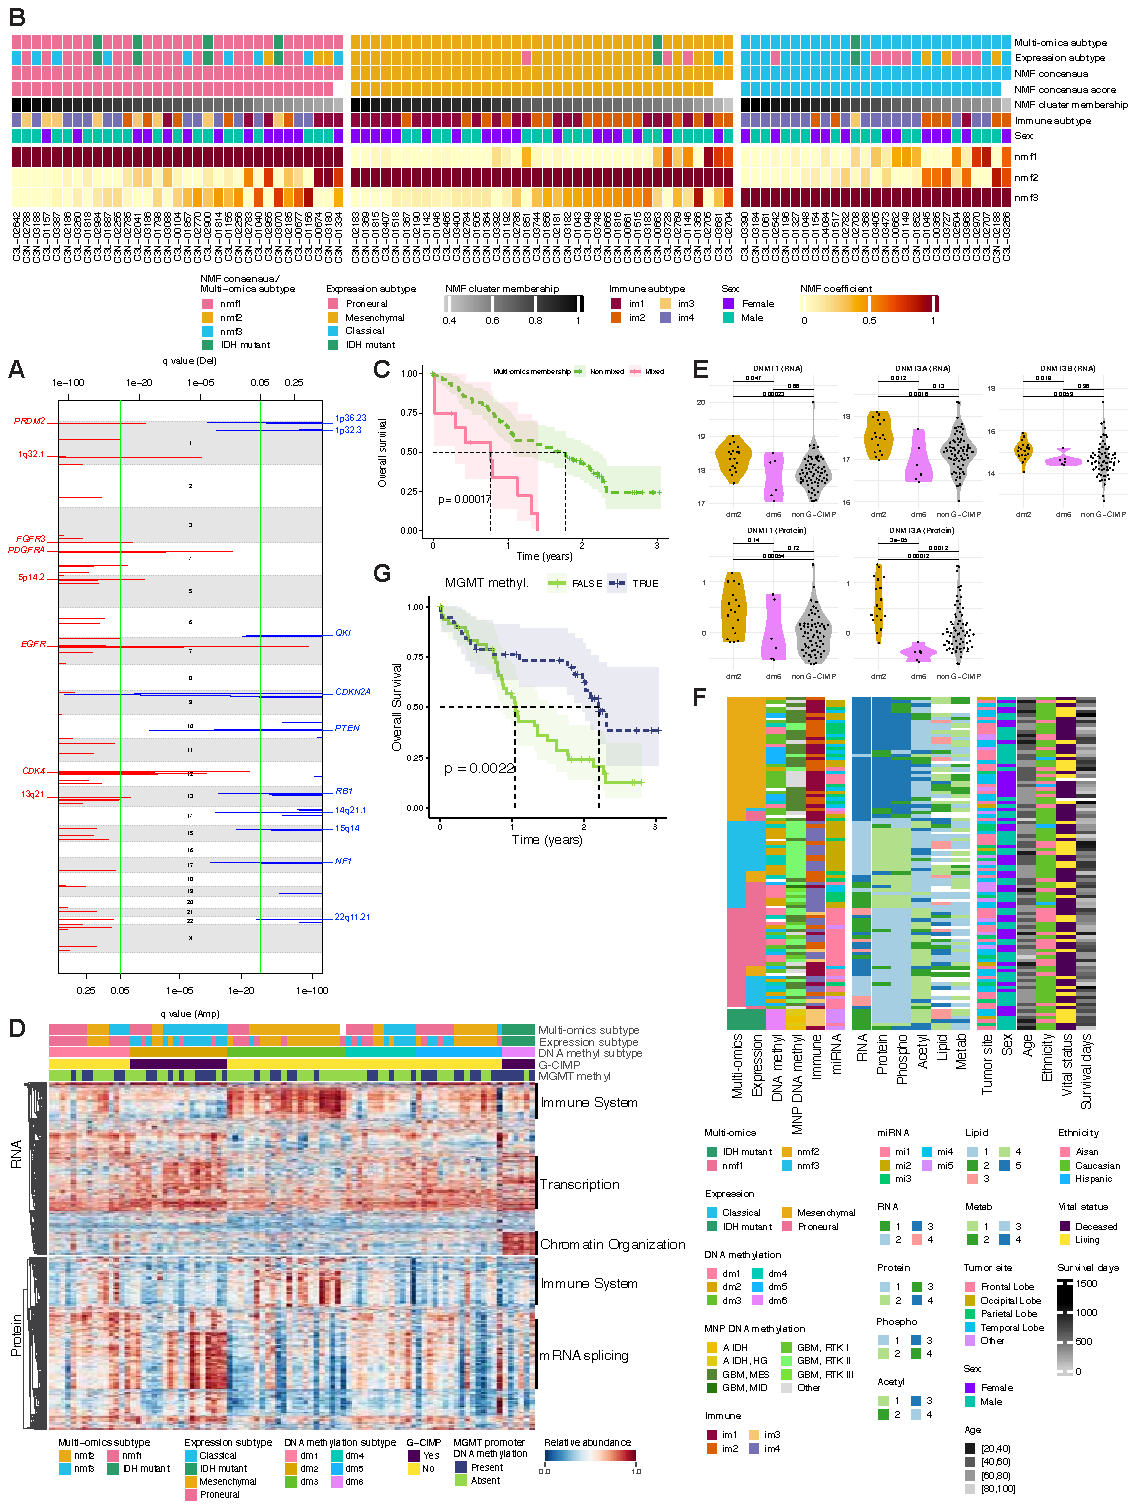
\includegraphics[width=0.95\linewidth]{figures/chap04_cptac_gbm_discov/figures2_subtypes.pdf}
    \caption[Proteogenomic Characterization and Subtyping of GBM.]{%
        Proteogenomic Characterization and Subtyping of GBM.
        \legendcontdnote
    }
    \label{fig:gbm-subtype}
\end{figure}
\begin{figure}[t]
    \centering
    \legend{%
        \legendcontdref{fig:gbm-subtype}
        \subref{fig:gbm-subtype-gistic}
        GISTIC2 copy number variations at and focal level of all tumors with WGS available.
        \subref{fig:gbm-subtype-nmf}
        Heatmap of multi-omics membership scores of all three multi-omics subtypes for each tumor.
        \subref{fig:gbm-subtype-mixed-subtype}
        Survival Kaplan–Meier curves of mixed-subtype tumors with low multi-omics membership score versus the rest of the tumors.
        \subref{fig:gbm-subtype-methyl}
        Pathway enrichment analysis of gene expression with differential DNA methylation in promoter regions across all six DNA methylation subtypes.
        \subref{fig:gbm-subtype-dnmt}
        Differentially expressed DNMTs in two G-CIMP subtypes (dm2 and dm6) at both RNA and protein level.
        \subref{fig:gbm-subtype-each-data-type}
        Comparison of the clustering results using individual data type, including DNA methylation, miRNAs, RNAs, proteins, phosphoproteins, acetylproteins, lipids, and metabolites.
        \subref{fig:gbm-subtype-mgmt-survival}
        Survival Kaplan--Meier curves of tumors with different MGMT promoter DNA methylation status.
    }
\end{figure}

Clinical data associated with the three subtypes indicated that tumors with relatively low multi-omics membership scores for two or more subtypes, i.e. those of ``mixed subtype'' (n = 12) (\fref{fig:gbm-subtype-nmf}) were associated with worse prognosis (log rank test p = 1.7e-4; \fref{fig:gbm-subtype-mixed-subtype}) compared with those of non-mixed subtype (excluding \gene{IDH1}-mutant tumors). We identified three proteins associated with poor survival across all tumors: low expression of HIST3H2BB (log rank test p = 0.0034), high expression of MT-CYB (p = 0.03), and high expression of PRODH (p = 0.096).
Genome-wide DNA methylation profiling identified six DNA methylation subtypes, including two distinct glioma CpG island methylator phenotype (G-CIMP) subtypes (dm2 and dm6). The dm6 subtype is IDH-mutant-specific with upregulation of chromatin organization pathways, while dm2 consists of \gene{IDH}-WT tumors with upregulation of transcription and mRNA splicing pathways (\fref{fig:gbm-subtype-methyl}).
Two subtypes showed elevated expression of different \textit{de novo} DNA methylases (\fref{fig:gbm-subtype-dnmt}). We also examined \textit{cis} associations of DNA methylation with RNA or protein abundances using iProFun \cite{songx_wangp:InsightsImpact2019}.
For example, 38 of 90 tumors (42\%) exhibited hypermethylation of the MGMT promoter region and significantly decreased MGMT RNA and protein levels (Welch's t test p = 4.9e-11 and 2.6e-6, respectively) (\fref{fig:gbm-subtype-mgmt-survival}).


\subsection{Driver genetic alterations influence oncogenic protein abundance and phosphorylation}


\section{Discussion}
